\chapter[Object-Oriented Design]{Object-Oriented\\ Design}
\label{chap:object_oriented_design}

% Position the image to the right of the heading.
\vspace{-9\baselineskip} % move up
\hfill
 \begin{minipage}{0.5\textwidth}
 \centering
 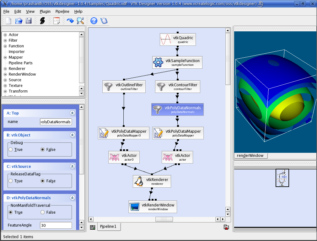
\includegraphics{VTKTextbook-10}
  \captionof*{figure}{\textit{VTK Designer image courtesy of vcreatelogic.com.}}
 \end{minipage}
\vspace{2\baselineskip}

\firstletter{O}bject-oriented systems are becoming widespread in
the computer industry for good reason. \\Object--oriented systems are more modular, easier to maintain, and easier to describe than traditional procedural systems. Since the \emph{Visualization Toolkit} has been designed and implemented using object--oriented design, we devote this chapter to summarizing the concepts and practice of object--oriented design and implementation.

\section{Introduction}

Today's software systems try to solve complex, real--world problems. A rigorous software design and implementation methodology can ease the burden of this complexity. Without such a methodology, software developers can find it difficult to meet a system's specifications. Furthermore, as specifications change and grow, a software system that does not have a solid, underlying architecture and design will have difficulty adapting to these expanding requirements.

Our visualization system is a good example of complex software that needs to be designed with extensibility in mind. Data visualization is a rapidly expanding field, with visualization techniques being introduced each year. Any system that hopes to incorporate future innovations must have an underlying design that supports the addition of new material without a significant impact on the existing system.

Object--oriented design is a software engineering methodology that deals comfortably with complexity and provides a framework for later changes and additions. The object--oriented design process attempts to divide a complex task into small and simple pieces called objects. The objects are computer abstractions that model physical or abstract pieces of the system being simulated. Object--oriented design methodologies provide mechanisms to identify the abstractions that exist within a system and to model the behavior of the objects.

\section{Goals of Good Software Design}

The quality of a software design is difficult to measure, but some qualitative aspects can guide us. A good software design should be robust, understandable, extendible, modular, maintainable, and reusable.

A robust system handles exceptional conditions gracefully and behaves consistently. Robustness gives software developers confidence that the underlying components of the system will behave as expected, even when the system is used under different circumstances than the original implementor intended.

An understandable system can be used by someone other than the original implementor. The use of the system should seem logical and sensible. The names of the components of the system should be derived from the problem domain.

Extendable systems accept new tasks while still doing the tasks they were originally intended to perform. A system should accept new forms of data and new algorithms without disrupting existing software. Adding a new primitive to the system should not cause large portions of the system to be modified. Experience shows that the more existing code that is modified in a system, the more likely errors will be introduced.

Modular software systems minimize the number of relationships that exist between components of a system. System components that are tightly coupled should be grouped together logically and obey common naming conventions and protocols.

Software maintenance is often ignored during system design. Nevertheless, the total cost of a system includes maintenance as well as the original development. A software system is maintainable if problems are easily isolated and the repair of one problem does not introduce problems in unrelated parts of the system.

Finally, the economics of software development require that we leverage as much of our past work as possible. In an ideal world, the implementation of a new technique in an existing system should be a simple task. This is seldom the case in software systems. Creation of reusable software components can reduce duplication of effort and promote consistent interfaces within a system. However, as we see throughout this book, creating software that can be reused often takes extra effort. A short--term view of productivity by one individual conflicts with the long--term view of the productivity of a software development organization.

\section{Object--Oriented Concepts}

Objects are the dominating concepts in object--oriented systems. Objects are abstractions that encapsulate the properties and behavior of the entities within a system. Each object has an identity that distinguishes it from other objects in the system. Often, the distinguishable aspects of an object are obvious. For example, a difference in color, location on a screen, size, or contents distinguishes one window from another on a computer desktop. But, appearances can be deceiving, and even two objects that share all the same characteristics may still have different identities. Two automobiles may have the same manufacturer, model, options and colors, but remain two different cars. The real world distinguishes the two cars by a vehicle identification number. Likewise, programming systems that deal with multiple entities need an identity mechanism. A pointer to allocated memory or a variable name in a system-managed symbol table are often used to distinguish objects in a system. In a database system, a set of identifier keys (called an \emph{n}--tuple) identifies an entity\index{entity} in a system.

But, how do object--oriented systems differ from conventional, procedural programming systems? The major difference is in the way the two approaches treat data abstraction. Conventional systems limit abstraction to data typing, while object--oriented systems create abstractions for both the data and the operations that can be applied to the data. In fact, an object--oriented system keeps the data and operations together in one programming construct called an object. Together, the data and operations comprise an object's \emph{properties}. When an operation is applied to an object, the programming language's dynamic-binding mechanism executes the procedure that is appropriate for that object. This is not the case in procedure--oriented systems. The programmer must supply logic to decide which procedure to call. Systems that handle multiple types are often littered with case statements to select the appropriate procedure for an operation. As new types are added to these systems, the code that dispatches operations based on data type must be extended to handle the new type. For example, in a program to display different types of primitives, the following pseudo code shows how a procedure-oriented system differs from an object--oriented system.

Procedure oriented (in C++):

\begin{lstlisting}[language=C++, caption={Procedure oriented.}]
Primitive *aPrim;
...
DrawPrimitive (aPrim)
...
procedure DrawPrimitive (aPrim)
{
  if (aPrim->type == TRIANGLE) then DrawTriangle (aPrim)
  else if (aPrim->type == SQUARE) then DrawSquare (aPrim)
  else if (aPrim->type == CIRCLE) then DrawCircle (aPrim)
...
}
\end{lstlisting}

Object--oriented (in C++):

\begin{lstlisting}[language=C++, caption={Object--oriented.}]
...
aPrim->Draw ();
...
\end{lstlisting}

Later in this project's existence, someone may want to add a new primitive, let's say a quadratic. The person assigned with such a formidable task must search the existing system for all occurrences of the if statements in the first example and add a test for the new quadratic type. Of course, a good programmer will have isolated the code in one location, as we have done here, so the task is easier. Nevertheless, that programmer must first realize that the original programmer was skilled enough to modularize the drawing code, then find the code (without necessarily knowing the procedure name) and modify the code. To complicate matters, a system built by more than one programmer will undoubtedly be under a configuration management system, requiring a check--out, edit, and check-in cycle.

The object--oriented programmer has an easier task. Consulting the design document that defines the object properties for a primitive, this programmer adds a draw operation to the quadratic object. The new primitive is available to the system without changing any existing code! Of course, this is an oversimplified example. But think about past programs you have written and remember how hard it was to add a new data type. Were your changes isolated to the new code you added? Did you have to edit code that you did not write and maybe did not understand? Keep this example in mind as you read our object--oriented implementation of a data visualization library.

Before describing object--oriented design and programming in more detail, we provide an observation and prediction. Over the several years that we have designed and implemented software using an object--oriented methodology, we have observed that newcomers to the technique will say, ``But this is how I already write programs. My systems are modular; they're robust; I can easily add to them''. If you still feel that way after reading this book, do not fault the object--oriented approach. Rather, we have failed as authors. However, such a negative response is unlikely. In our experience, users become comfortable with this approach in a short time. Especially when they are introduced to objects through an existing, well-designed object--oriented system. You will reach the ``aha'' stage, after which it will be difficult to begin a software project without looking for the objects in the problem.

\section{Object--Oriented Terminology}

As with any software engineering design methodology, object--oriented design has its own terminology. Unfortunately, not everyone agrees on what that is. We adopt much of our terminology from Rumbaugh \cite{Rumbaugh91} and, since the \emph{Visualization Toolkit} is written in C++, from Stroustrup \cite{Stroustrup84}. For the most part, Rumbaugh's terminology is independent of programming language, while Stroustrup is specific to implementation in C++. The transition from design to programming will be painless though, and the mappings between the two terminologies are mostly obvious. Where we think there might be confusion, we will point out the correspondences.

\subsection{What Is an Object?}

An \emph{object} is an abstraction that models the state and behavior of entities in a system. Abstraction\index{abstraction} is a mental process that extracts the essential aspects of a situation for a particular purpose. Entities are things in the system that have identity. Chairs, airplanes, and cameras are objects that correspond to physical entities in the real world. Binary trees, symbol tables, and ordered collections are objects that exist only within the world of computer science.

Figure \ref{fig:Figure2-1} is an example of the abstraction that occurs when we map the state and behavior of a system component to an object. Here, the object is a particular type of tree: a pin oak. In this application we desire to simulate the growth of various types of trees over the course of a season. For our purpose we have decided that the important state variables are the tree's age, trunk diameter, height, and habit (i.e., growing form). To capture the behavior of the pin oak we have methods to simulate growth and seasonal effects corresponding to spring, summer, fall, and winter. There are also methods (not shown) for setting and getting current state variables.

\begin{figure}[!htb]
	\centering
	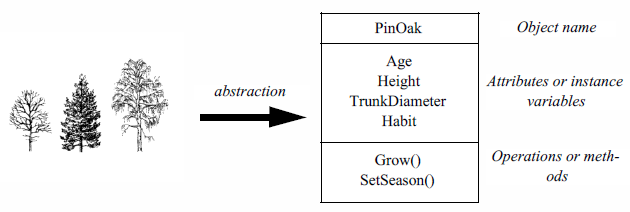
\includegraphics[width=0.8\textwidth]{Figure2-1}
	\caption{Mapping a real-world object into an object abstraction. The real-world objects are various types of trees. One of these objects (a pin oak tree) is mapped into the computer object we call PinOak.}
	\label{fig:Figure2-1}
\end{figure}

We call the state of an object its \emph{attributes}\index{attribute} (also called \emph{instance variables} ) and define its behavior by the \emph{operations} that can be applied to it. Attributes have a name, a data type, and a data value. The data type of an attribute may be a primitive type in the programming language (such as a char or float in C++), or another object. For example, the vtkTransform object in our visualization system has an attribute of type vtkMatrix4x4 , another object. vtkMatrix4x4 in turn has attributes that are an array of primitive values declared as float values in C++.

Operations are functions or transformations that can be applied to an object. Operations define the behavior of the object. The operations for a particular object are implemented in procedures we call \emph{methods}.

Together, the attributes and operations of an object comprise its \emph{properties}. A two--dimensional line graph could have attributes that include an \emph{x} and \emph{y} axis, a legend, and a connected set of points. This graph has methods that draw the graph in a window. It also has methods that let a user specify the axes, data to draw, and legend to use.

Objects that share the same properties can be grouped using the process of \emph{classification}\index{classification}. An object class, usually just called a class, specifies the properties that all objects in the class have. The class only specifies the names of the properties, not their specific values. Different classes can (and usually do) have properties with names that exist in other classes. Many classes in our visualization system have an attribute named Position. Although both a camera and actor in our visualization system have this attribute, the effect on each is different because they are different classes. Attribute names are shared by all objects in a given class, but separate storage is allocated for each object's attribute values.

When an operation with the same name is applied to objects of different classes we call the operation \emph{polymorphic}. For example, our visualization system has an operation named Render() that can be applied to many different objects. The implementation of an operation for a particular class is called a method. The print operation for a vtkMatrix4x4 object is implemented in its print method. That is, there exists code that knows how to print objects of class vtkMatrix4x4 and not objects of other classes. Objects know which method to use because they are kept within each object's data structure. In most systems the code for the methods is shared by all objects in the same class. Some programming languages, including C++, define a method by combining an operation name with its argument types. This process is called overloading an operation and is a powerful technique that permits the same name to be used for logically similar operations. For example, the class definition below defines three methods for calculating the square of a number. Even though these methods have the same operation name, they are unique because C++ uses both the operation name and the operations argument types.
\index{classification!example}

\begin{lstlisting}[language=C++, caption={math class.}]
class math
{
  float square(float x);
  int square(int x);
  double square(double x);
}
\end{lstlisting}

To use a member of a class for some purpose, we create an instance of the class (the process of \emph{instantiation}). Instance creation establishes the identity of the instance including specifying its initial state. The instance's class serves as a template for the instance during creation, defining the names of each of its attributes and operations. Creation establishes the similarities and differences between this instance and other instances of the same class. The similarities are the names and type of its attributes and the methods that implement its operations. The differences are the specific values of the attributes. The details of how one creates an instance of a class vary from programming language to programming language. In C++, a program creates an instance using a declarative form such as

\begin{lstlisting}[language=C++,  caption={}, numbers=none, frame=none]
vtkActor aBall;
\end{lstlisting}

\noindent which creates an object from the program stack, or by applying the new operation

\begin{lstlisting}[language=TCL,  caption={}, numbers=none, frame=none]
vtkActor *aBall = new vtkActor;
\end{lstlisting}

\noindent which creates the object from the program heap.

\subsection{Inheritance}
\emph{Inheritance} is a programming mechanism that simplifies adding new classes to a system when they differ in small ways from currently existing classes. The notion of inheritance is adopted from the observation that most systems can be specified using a hierarchical classification system. A fine example of a classification system is the phyla of life on earth.

Earlier we created an object corresponding to a pin oak tree. The properties of the tree can be more thoroughly described using inheritance (Figure \ref{fig:Figure2-2}). The classification shown here is based on the five kingdom system of Margulis and Schwartz \cite{Margulis88}.
In this system, biota is classified as belonging to one of the five kingdoms Prokaryotae (bacteria), Protoctista (algae, protozoans and slime molds), Fungi (mushrooms, molds, lichens), Plantae (mosses, ferns, cone--bearing, and flowering plants), and Animalia (animals with and without backbones). Below this level we have the classifications division, class, order, family, genus, and species. The figure shows the kingdom, division, class, genus, and species of the pin oak.

\begin{figure}[!htb]
	\centering
	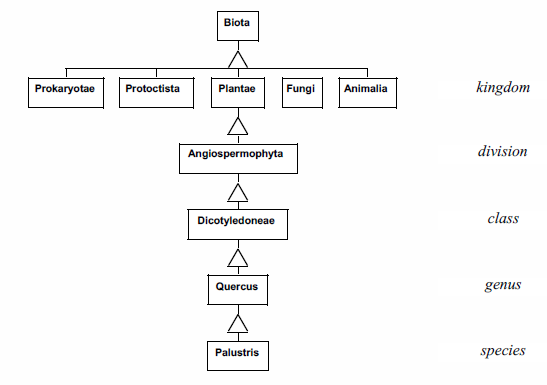
\includegraphics[width=0.8\textwidth]{Figure2-2}
	\caption{Inheritance hierarchy for pin oak tree.}
	\label{fig:Figure2-2}
\end{figure}

Organizing objects into an inheritance hierarchy provides many benefits. Properties of a general classification are also properties of its subclassification. For example, we know that all species of genus \emph{Quercus} form acorns. From the software point of view this means any instance variables and methods of a \emph{superclass}\index{class!superclass} are automatically inherited by its \emph{subclass}\index{class!subclass}. This allows us to make changes to a number of objects simultaneously by modifying their superclass. Furthermore, if we desire to add a new class (say a red oak tree) to the hierarchy we can do so without duplicating existing functionality. We need only differentiate the new class from the others by adding new instance variables or overloading existing methods.

The ability to quickly add new classes that are slightly different from currently existing classes promotes the extensibility of a system. Inheritance can be derived top--down using a process called \emph{specialization} , or it can be created bottom-up, combining similar classes during a process called \emph{generalization}\index{generalization}. The use of inheritance implies a class hierarchy with one or more classes being the superclasses of one or more subclasses. A subclass inherits the operations and attributes of its superclasses. In C++, subclasses are called \emph{derived}\index{class!derived}\index{derived class} classes and superclasses are called \emph{base} classes\index{base class}\index{class!base}. A subclass can add additional operations and attributes that modify the properties it inherited from its superclasses. Through this inheritance, an object can exhibit its superclass's behavior plus any additional behavior it wishes. It can also restrict, or override, operations implemented by its superclass.

Classes that exist only to act as superclasses for their subclasses are called \emph{abstract} classes\index{abstract class|(}\index{class!abstract|(}. Instance creation of an abstract class is generally prohibited. Abstract classes are useful for gathering attributes and methods that all subclasses will use. They can also define protocols for behavior for their subclasses. This is a powerful use of inheritance that will show up in the design of our visualization system. Abstract classes can enforce complex sequence, control protocols, and ensure uniform behavior. They remove the responsibility of complex protocols from the individual sub--classes and isolate the protocol in the superclass.

An example of a simple plotting package illustrates the power of abstract classes. Consider a data presentation application that allows for a variety of two--dimensional plotting. This application must support line charts and horizontal and vertical bar charts. The design process identifies properties common to all plots including title, axes, and legend. We then create an abstract class called TwoDPlot to contain these common attributes. Common behavior can also be captured in TwoDPlot within its plot method:

\begin{lstlisting}[caption={TwoDPlot.}]
Method Plot
{
  Draw the border
  Scale the data
  Draw the axes
  Draw the data
  Draw the title
  Draw the legend
}
\end{lstlisting}

An abstract class may or may not provide default behavior for each operation. In this example, default behavior for border and title drawing might be provided. Then subclasses of TwoDPlot would define their own functions for the other methods\index{abstract class!and subclass}. The protocol specification explicitly spells out what methods a subclass of TwoDPlot should respond to. In the above example, subclasses will need to define their own methods for drawing the axis, data, and legend. Some subclasses might use TwoDPlot 's methods for drawing the border, others might require their own version of this method. The abstract interface defined in TwoDPlot makes it easier to add new classes of 2D plots and the resulting subclasses tend to be more uniform and consistent.

Another mechanism, \emph{delegation}\index{delegation}, is useful for isolating and reusing behavior. Using delegation, an object applies operations to one of its attributes that is an object. As an example, in the \emph{Visualization Toolkit} the vtkTransform object delegates its Identity() operation to its vtkMatrix4x4 attribute. This instance of vtkMatrix4x4 then performs the operation. There are many more useful object--oriented concepts, but for the time being we have enough information to describe how we can use objects to design a system.

\section{Object--Oriented Modelling and Design}
\index{abstraction!during design}

The design of any large software system is a formidable task and the first steps in system design are often the most challenging. No matter what design technique we choose, we must have a thorough understanding of the system's application domain. It would be difficult to see how one could design a fly--by--wire airplane control system without a detailed knowledge of the underlying hardware control systems. Of course, all flight system software is not designed by aeronautical engineers, so some form of system specification must exist. The depth of information in the specifications varies from application to application.

Object--oriented system design begins with a modelling step that extracts objects and their relationships with other objects from a problem statement or software requirement specification. First, the designer must completely understand the problem being solved. This often requires an in-depth knowledge of the problem domain or access to detailed specifications of the problem being solved. Then, major abstractions must be identified within the system. The abstractions will become, at this high level of design, the first set of objects. For example, a system that keeps track of an investment portfolio will need objects such as stocks, bonds, and mutual funds. In a computer animation system we might need actors, cameras, and lights. A medical computed tomography system will have a table, X-ray source, detectors, and gantry. Our visualization system will have models, isosurfaces, streamlines, and cut planes. During this modelling step, we search the problem domain for objects, properties, and relationships. Later, during multiple passes through the design, the model will be expanded.

Modelling is a step in most design processes regardless of whether we are designing a ship, house, electronics system, or software. Each discipline follows a methodology that uses techniques specifically created to make the design process efficient and worthwhile. These techniques are so--called ``tools of the trade''. An electrical engineer uses schematics and logic diagrams, an architect uses drawings and mock-ups, and a ship builder uses scale models. Likewise, software designers need tools that can help create a model of the system. The software tools should have enough expressive power to help the software designer evaluate a design against a specification and help communicate that design to others on the software team.

We use the Object Modeling Technique (OMT) developed at GE by Jim Rumbaugh and his colleagues \cite{Rumbaugh91}. OMT uses three models to specify an object--oriented design: an object model, a dynamic model, and a functional model. Each model describes a different aspect of the system and each has a corresponding diagramming technique that helps us analyze, design, and implement software systems.

\subsection{The Object Model}

The object model\index{class!in object model} identifies each object in the system, its properties, and its relationships to other objects in the system. For most software systems, the object model dominates the design. The OMT graphical technique uses rectangles to depict object classes, and a variety of connectors to depict inheritance and other object--object relations. Object classes are represented as solid rectangles. Instances are represented as dotted rectangles. The name of the class or instance occupies the top of the rectangle. A line separates the class name from the next section that contains the attributes; a third section describes the methods. Relationships between objects are shown with line segments connecting the two related objects. In OMT, relationships are called associations and they can have various cardinalities: one-to-one, one-to-many, and many-to-many. Special associations that represent containers of other objects are called aggregations. Associations\index{association!in object model} can be labeled with roles. (Roles are names given to associations and are used to further describe the nature of the association.) OMT represents inheritance with a triangle, with the superclass attached to the apex, and sub-classes attached to the base of the triangle. Figure \ref{fig:Figure2-3} shows an object model for locator devices in a virtual reality system.

\begin{figure}[!htb]
	\centering
	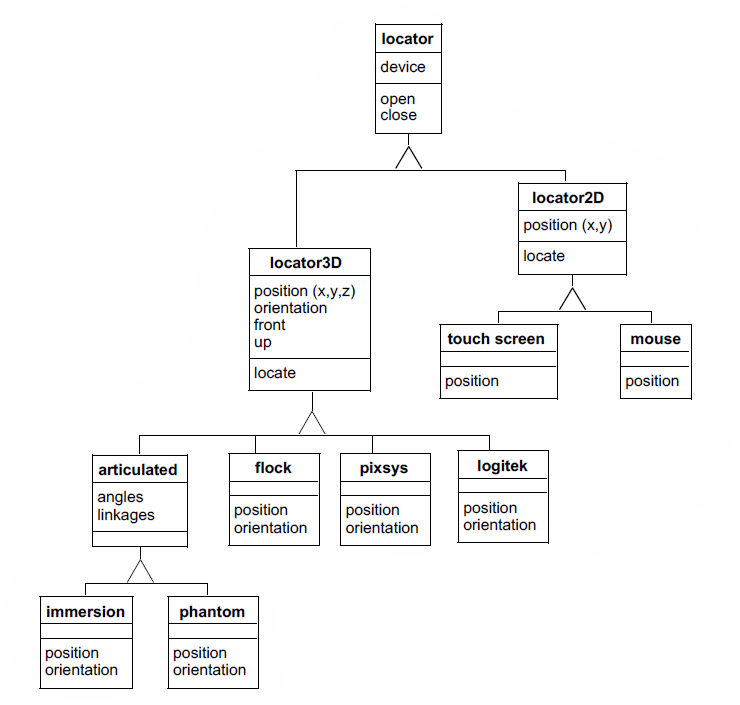
\includegraphics[width=0.8\textwidth]{Figure2-3}
	\caption{Object model for locator devices.}
	\label{fig:Figure2-3}
\end{figure}

The first object in the class hierarchy is locator. This abstract class specifies common attributes and methods for all locators\index{abstract class!example}. The subclasses of locator are locator2D and locator3D. In  the current rendition of this object model, the locator only has one attribute, a device and two methods, open() and close(). The two subclasses of locator, locator2D and locator3D are also abstract classes, containing attributes and methods that distinguish them from each other based on their spatial dimensionality. For example, locator3D has an \emph{x, y, z} position while locator2D has an \emph{x, y} position. Both locators have a locate() method that updates the current position. In the 3D locator class, locate() also updates the orientation. The subclasses of locator3D include hardware from three different manufacturers: flock, pixsys, and logitek, as well as an articulated positioner abstract class. The three object classes for the hardware contain methods specific to each device. Each method knows how to convert the hardware specific codes returned by the device. They know that to be considered a locator3D subclass, they must implement a position and orientation operation that will provide \emph{x, y, z} coordinates and three angular rotations that can be composed into a transformation matrix. The object model also shows us that the articulated locator has angles and linkages. Two specific articulated locators are immersion and phantom. An object model diagrammed in this fashion serves as a starting point for design and discussion. It reveals common methods and attributes as well as the distinguishing characteristics of each class.

Later, during implementation, we will convert these object models into software objects. The particular computer language we choose for implementation will dictate the details of the conversion.
\index{abstract class|)}\index{class!abstract|)}

\subsection{The Dynamic Model}
\index{dynamic model|(}

The object model describes the static portion of a system while the dynamic model details the sequences of events and time dependencies of the system. OMT uses state diagrams to model system dynamics. Dynamic models are frequently used to design control systems and user interfaces. Our visualization system has limited sequence and control aspects, so we will not dwell on state diagrams. But, if we were designing a user-friendly interface for a digital wristwatch, the state diagram in Figure \ref{fig:Figure2-4} would be useful.

\begin{figure}[!htb]
	\centering
	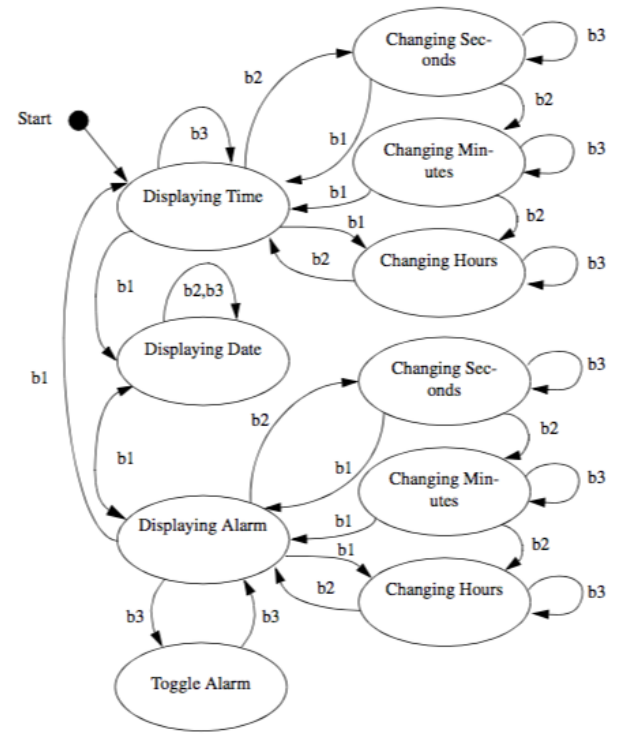
\includegraphics[width=0.8\textwidth]{Figure2-4}
	\caption{State diagram for a wristwatch.}
	\label{fig:Figure2-4}
\end{figure}

The ovals in the diagram show a state; the arrows show a transition from one state to another; and the labels on the arrows show an event that causes the state transition. This example shows three display states and multiple setting states. The event b1 means button one is pressed. This watch has three buttons. The diagram shows what happens in each state when any of the three buttons is pressed. The diagram clearly shows that b1 is used to move between display modes for time, date, and alarm. B2 changes from display mode into setting mode or selects the field to change in a given mode. B3 increments the selected field by one unit. The state diagram also shows what happens when illegal buttons are pressed. If the watch is displaying time and button 3 is pressed, nothing happens. If button 3 is pressed when the watch is displaying the alarm, the alarm on/off is toggled.
\index{dynamic model|)}

\subsection{The Functional Model}
\index{functional model}

The functional model shows how data flows through the system and how processes and algorithms transform the data. It also shows functional dependencies between processes. Exposing these relationships will affect the associations in the object model. The major components of a data flow diagram\index{data flow diagram} (DFD) are data sources, data sinks, and processes. Data sources and sinks are represented as rectangles. Ellipses show processes. Data stores are shown within two horizontal lines. DFDs are useful to describe the overall flow in the system. They can also be used to describe any process that transforms one data representation into another. Processes identified in the DFD during function modelling may turn up as operations or objects in the object model.

Figure \ref{fig:Figure2-5} shows a data flow diagram for a 3D medical imaging system. The diagram shows the data acquisition on the computed tomography (CT) or magnetic resonance imaging (MRI) scanner. The series of cross-sectional slices provided by the scanner is first processed by image processing filters to enhance features in the gray scale slices. A segment process identifies tissues and produces labels for the various tissues present in the slices. These labeled slices are then passed through a surface extraction process to create triangles that lie on the surface of each tissue. The render process transforms the geometry into an image. Alternatively, the write process stores the triangles in a file. Later, the triangles can be read and rendered into an image. We defer the decision whether to make the processes objects or operations until later. Chapter \nameref{chap:visualization_pipeline} uses DFDs to model the visualization pipeline.

\begin{figure}[!htb]
	\centering
	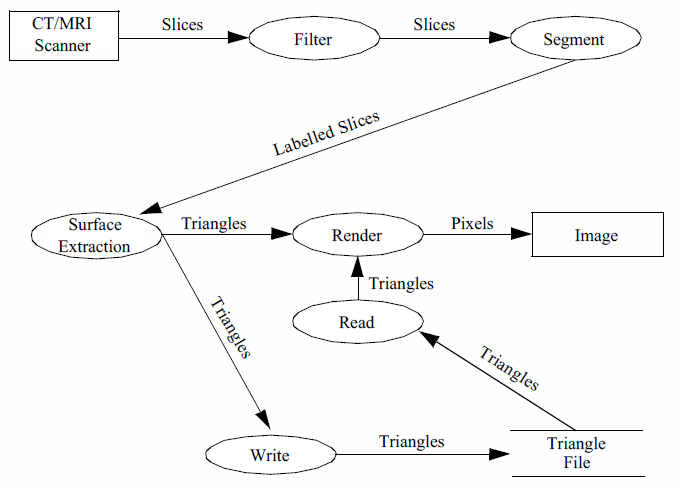
\includegraphics[width=0.8\textwidth]{Figure2-5}
	\caption{Data flow diagram.}
	\label{fig:Figure2-5}
\end{figure}

\section{Object--Oriented Programming Languages}

The choice of computer programming language is a religious issue. Every computer language has its evangelists and followers. Most of our experience in object--oriented languages is with C and C++\index{C++}. C itself does not have object--oriented facilities, but an object--oriented methodology and strict coding guidelines permit the development of object--oriented code. We chose C++ for the \emph{Visualization Toolkit} because it has built-in support for the notion of classes, dynamic binding of methods to objects, and inheritance. C++ is also widely available on many UNIX platforms and personal computers.

Simula \cite{Birtwistle79} is usually acknowledged as the first object--oriented language, but Smalltalk \cite{Goldberg83} is probably the best-known language. Smalltalk was developed at the Xerox Palo Alto Research Center (PARC) in the seventies and eighties. Well before its time, Smalltalk provided not just a language, but also an operating system and programming environment built with objects. When you use Smalltalk, you live and breathe objects. For the object--oriented purist, there is no substitute. Smalltalk spin-offs include window systems, workstations, and the desktop paradigm. Both Apple Computer and Microsoft acknowledge the influence that Smalltalk and Xerox PARC had on the Macintosh and Windows. Smalltalk was probably conceived 10 years too early for widespread commercial acceptance. During Smalltalk's infancy and adolescence, the complexity of software was much lower than today's systems. FORTRAN served the scientific and engineering community, COBOL was the choice for business applications and the computer science community embraced C. The use of abstractions was limited to mathematicians and other abstract thinkers. Programming was considered an art form and programmers concentrated on clever implementations of algorithms. Each new task often required a new program. Technical programmers did use numerical libraries for common mathematical operations, but any notions of common abstractions at a higher level were relatively few.

\section{Object--Oriented Visualization}

Don't underestimate the investment required to design a system. Although object--oriented technologies have tremendous potential to produce good software designs, these techniques do not guarantee a good design. The visualization system we present in this text has its roots in an animation \cite{Lorensen89} and visualization system \cite{Schroeder92} that we developed over a 10-year period. The initial design, which identified 25 classes for computer animation of industrial applications, took four software professionals 10 months (almost 3.5 person years) to complete. During this design stage the developers produced zero (!) lines of code. The subsequent implementation took one month, or ten percent of the effort. This system still serves our visualization group even after 20 other software developers have added over 500 classes to the system. The original 25 classes still exist in the system today.

As a reader, we hope that you can benefit from our experience in visualization system design. We have tried to assist you by describing the properties (attributes and methods) of many of the \emph{Visualization Toolkit} classes in each chapter's ``Putting It All Together'' section. There are also included a series of object diagrams generated by the Doxygen documentation system that will give you a quick overview of object relationships such as superclass and subclass. This documentation can be found on the CD--ROM or on--line at \href{https://www.vtk.org/doc/nightly/html/index.html}{VTK Documentation}. In the next chapter we will also explain the decisions we made to design the VTK object--oriented toolkit.

\section{Chapter Summary}

This chapter introduced object--oriented concepts and terminology. The emphasis was on dealing with complexity and how object--oriented technology provides mechanisms to reduce the complexity of software.

Model building is an important part of any design methodology. We introduced three models and notations. The object model describes the objects in a system and their static relationships, attributes, and methods. Object diagrams succinctly present this static information. The dynamic model focuses on the time dependent aspects of the system. State transition diagrams are used to model the sequence and control portions of the system. The functional model shows how objects in the system transform data or other objects. The data flow diagram is a convenient notation for showing functional dependencies.

There are several choices available today for object--oriented implementations. Although it is possible to implement an object--oriented system in a non--object--oriented language such as C, the methodology is best served by an object--oriented language. We have chosen C++ to implement the \emph{Visualization Toolkit}.

The emphasis in this book is on architecture, data structure design, and algorithms. The object--oriented aspects of the system are important, but what the system does is far more important.

\section{Bibliographic Notes}
There are several excellent textbooks on object--oriented design.
Both \cite{Rumbaugh91} and \cite{Birtwistle79} present language-independent design methodologies.
Both books emphasize modelling and diagramming as key aspects of design.
\cite{Meyer88} also describes the OO design process in the context of Eiffel, an OO language.
Another popular book has been authored by Booch \cite{Booch91}.

Anyone who wants to be a serious user of object--oriented design and implementation should read the books on Smalltalk \cite{Goldberg83} \cite{Goldberg84} by the developers of Smalltalk at Xerox Parc.
In another early object--oriented programming book, \cite{Cox86} describes OO techniques and the programming language Objective--C.
Objective--C is a mix of C and Smalltalk and was used by Next Computer in the implementation of their operating system and user interface.

There are many texts on object--oriented languages. CLOS\index{CLOS} \cite{Keene89} describes the Common List Object System. Eiffel\index{Eiffel}, a strongly typed OO language is described by \cite{Meyer88} .
Objective-C \cite{Cox86} is a weakly typed language.

Since C++\index{C++} has become a popular programming language, there now many class libraries available for use in applications.
\cite{Gorlen90} describes an extensive class library for collections and arrays modeled after the Smalltalk classes described in \cite{Goldberg83} .
\cite{Stepanov94} and \cite{Musser94} describe the Standard Template Library, a framework of data structures and algorithms that is now a part of the ANSI C++ standard. Open Inventor \cite{Inventor} is a C++ library supporting interactive 3D computer graphics.
The Insight Segmentation and Registration Toolkit (ITK) is a relatively newclass library often used in combination with VTK \cite{ITK} for medical data processing. VXL is a C++ library for computer vision research and implementation \cite{VXL}.
Several mathematical libraries such as VNL (a part of VXL) and Blitz++ \cite{Blitz} are also available. A wide variety of other C++ toolkits are available, Google searches \cite{Google} are the best way to find them.

C++ texts abound. The original description by the author of C++ \cite{Stroustrup84} is a must for any serious C++ programmer. Another book \cite{Ellis90} describes standard extensions to the language.
These days the UML book series --- of which \cite{Booch98} and \cite{Rumbaugh98} are quite popular --- are highly recommended resources. Several books on generic programming \cite{Austern99} and STL \cite{Musser96} are also useful. Check with your colleagues for their favourite C++ book.
To keep in touch with new developments there are conferences, journals, and Web sites. The strongest technical conference on object--oriented topics is the annual Object--oriented Programming Systems, Languages, and Applications ( OOPSLA ) conference. This is where researchers in the field describe, teach and debate the latest techniques in object--oriented technology. The bimonthly Journal of Object-Oriented Programming (JOOP) published by SIGS Publications, NY, presents technical papers, columns, and tutorials on the field. Resources on the World Wide Web include the Usenet newsgroups comp.object and comp.lang.c++.

\printbibliography

\section{Exercises}

\begin{enumerate}
	\item Answer the following questions about a program you have written.
	\begin{enumerate}
		\item How much time did you spend on design and implementation?
		\item What methodology, if any, did you use?
		\item Could you easily extend the system?
		\item Could anyone extend the system?
	\end{enumerate}

	\item \label{exercise:2.2} Identify the major objects and operations for the following
	applications.
	\begin{enumerate}
		\item An airline reservation system.
		\item An adventure game.
		\item A 2D plotting package.
		\item An automatic teller machine.
	\end{enumerate}

\item Draw an object diagram for each example in Exercise \ref{exercise:2.2}.

\item \label{exercise:2.4}Computer animation uses concepts from graphics and movie making. Identify the major objects and operations in a computer animation system.

\item For the animation system in Exercise \ref{exercise:2.4}, design control and looping objects that will allow flexible control of the properties of the actors in the system. If we call these control and looping objects scenes and cues, how would you expect them to look?

\item Draw a state diagram for your wristwatch using Figure \ref{fig:Figure2-4} as an example.

\item Draw a data flow diagram for calculating the surface area and volume of a sphere and cylinder.

\end{enumerate}